\section{Harvest and Loading Processes as a Use Cases for \acl{WIC}}
The Forage harvester has proven to be an essential agricultural machine for harvest-
ing and loading forage. \textcite{seifert_feldhacksler_1962} define a forage harvester
as an agricultural loading machine for nearly all types of animal feed. By mounting different cutting and loading devices, a forage harvester can load the following animal feed, according to the authors: Hey, Straw, Corn, Grass and Clover.

\begin{figure}%
	\centering
	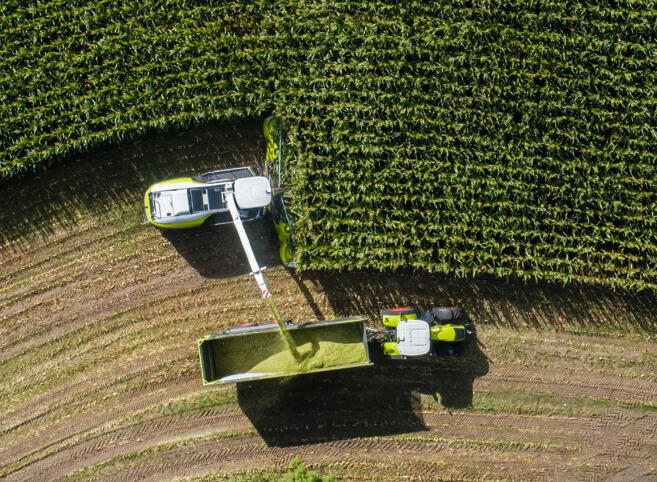
\includegraphics[width=0.6\textwidth]{figures/claas_harvest_side.png}
	\caption{\ac{FH} and \ac{TM} while }%
	\label{fig:normal}%
\end{figure}

In the harvesting and loading process, a \ac{TM} typically drives alongside or behind the \ac{FH} so that the \ac{FH} can load the harvested goods onto the trailer of the \ac{TM} using the spout. Drivers operate both machines and try to keep the speed and distance so that the spout only throws the harvested goods into the trailer of the TM. An image of a harvesting and loading process for corn can be seen in \autoref{fig:normal}.

Taking a corn harvest scenario as an example, key figures can be looked up in \cite{faustzahlen2018}, a standard reference book in agricultural literature. This book contains key figures of agricultural processes, which 80 experts have compiled. The key figures, which are shown in \autoref{tab:DataSilageHarvest}, are dependent on the \ac{PPD} and show the large amount of forage harvested by  a  \ac{FH} every hour.
\begin{table}
	\centering
	\begin{tabular}{>{\raggedright}p{5.5cm}p{1.6cm}p{1.6cm}p{1.6cm}}
		\toprule
		Kennzahlen & \ac{PPD} \SI{20}{\tonne\per\hectare} & \ac{PPD} \SI{30}{\tonne\per\hectare} & \ac{PPD} \SI{50}{\tonne\per\hectare}\\
		\midrule
		Required \ac{TM}s & \num{5}&
		\num{7} & \num{10} \\
		Harvesting performance volume [\si{\cubic\metre\per\hour}] &
		\num{285.7}-\num{333.3}
		& \num{428.6}-\num{500.0} &
		\num{595.7}-\num{695.0}\\
		Harvesting performance \ac{TM} loads [\si{\per\hour}] &
		\num{5.7} - \num{6.7}
		& \num{8.6} - \num{10.0} &
		\num{11.9} - \num{13.9}\\
		Harvesting performance mass [\si{\tonne\per\hour}] & \num{100}
		& \num{150} &
		\num{208.5} \\
		\bottomrule
	\end{tabular}
	\caption{Key figures from \cite{faustzahlen2018} of corn harvest of a \ac{FH} with a working width of \SI{6.2}{\metre} in a \SI{80}{\hectare}-field in regard to \ac{PPD}}
	\label{tab:DataSilageHarvest}
\end{table}

The harvesting and loading processes are examples of the use of an agricultural Platooning Services as described by 
\textcite{zhang_method_2009}.
This Platooning Service creates a leader and follower system where an uncrewed agricultural machine follows a leading operated agricultural machine.
For the harvesting and loading process, a Platooning service could be used as follows.
The operated \ac{FH}, as a leader, sets the path and speed and transmits the data via \ac{WIC} to the \ac{TM}. Based on the path and speed data of the \ac{FH}, \ac{TM} follows unmanned with a longitudinal and lateral offset, as \autoref{fig:offset} displays.
\begin{figure}%
	\centering
	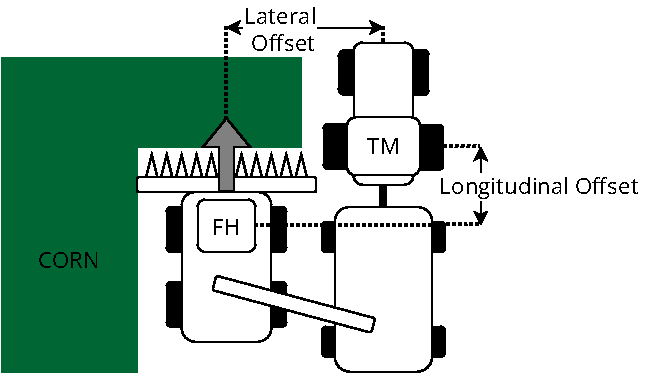
\includegraphics[width=0.65\textwidth]{figures/offset_platoon.pdf}
	\caption{Lateral and longitudinal Offset between the two agricultural machines \ac{FH} and \ac{TM} in a corn harvest scenario}%
	\label{fig:offset}%
\end{figure}

This Platooning Service positions the \ac{TM} optimally to the \ac{FH} so that the forage can be loaded ideally from the \ac{FH} onto the \ac{TM}.


\autoref{fig:workforce_agri} shows that the number of workers in the agriculture domain is declining.  
Because fewer and fewer workers are working in agriculture, the use of platooning services for harvest and loading processes can save and free up labour for other activities \cite{liu_automation_2022}.

As stated in \autoref{tab:DataSilageHarvest}, already ten drivers for the \ac{TM}s are needed in the corn harvest process with a high \ac{PPD}. 

Using an agricultural Platooning Service, each \ac{TM} can drive unmanned in the field leading to a smaller number of workers needed in the corn harvest process.

\textcite{IVAN} fügt dazu hinzu, dass Platooning Services auf Platoonebene die fahrer entlasten können, sodass diese sich auf das optimale Einstellen der Arbeitsmaschinen fokusieren können. Zusätzlich können \ac{TM}s zielgerichtet zu den \ac{FH} geführt werden, sodass die Logistikprozesse auf dem Feld verbessert werden können. ´

\begin{figure}%
	\centering
	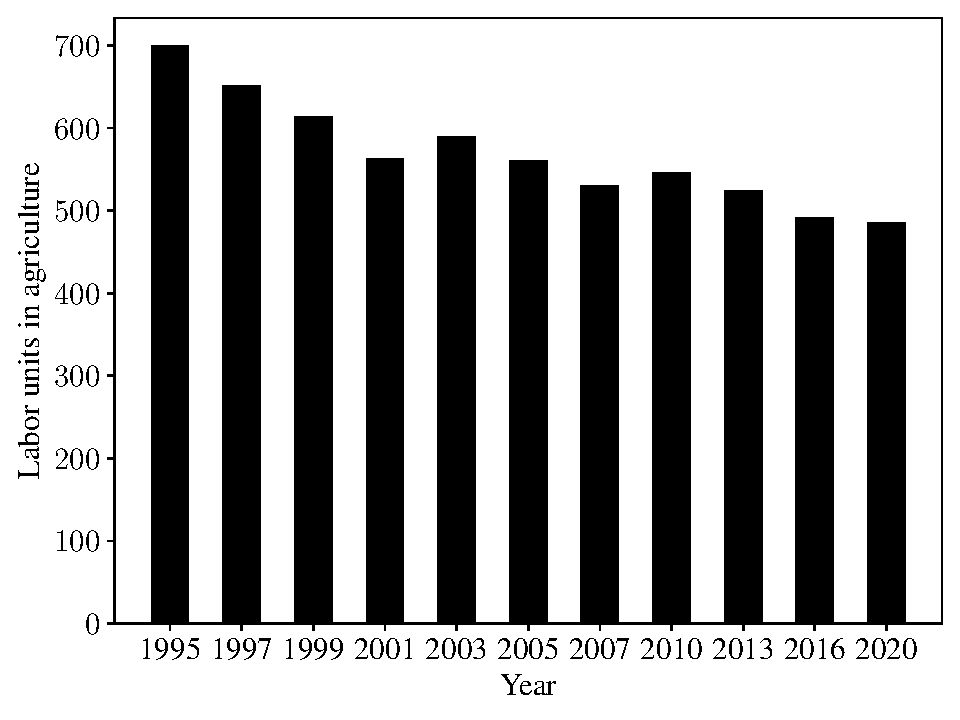
\includegraphics[width=0.75\textwidth]{figures/WorkForceAgriculture.pdf}
	\caption{Decrease in the agricultural labor force in Germany based on the data from \cite{bmel2020}}%
	\label{fig:workforce_agri}%
\end{figure}


At the same time, the harvest and loading processes are examples of the video streaming \ac{WIC} use case. During these harvest and loading processes the spout of the \ac{FH} must be controlled to set the loading position of the forage into the trailer of the \ac{TM}.

According to \textcite{murcia_quadrotor_2014}, different spout guidance and control systems have been developed to automate the filling of the trailer. Spout guidance and control systems use a camera attached to the spout to determine the fill volume at each point of the trailer via machine vision and set the spout to fill the empty parts of the trailer accordingly. The author describes Autofill - systems from Claas and Intellifill - systems from CNH Industrial as examples of spout guidance systems. 

Streaming the video of a camera at the spout from the \ac{FH} to the \ac{TM} would be a practical application of the video streaming use case in the harvesting process. If the \ac{TM} driver can watch a live stream of the trailer's fill level, he will always be
informed and knows when the trailer is full and can drive the forage back to the
farm.

\chapter{Analyzing Corn Harvest Process Data}

To gain a better insight into requirements of the \ac{WIC} use cases Platooning and Streaming Services, I analysed process data of a corn harvest scenario as the example for I collected GPS tracks of  a  \ac{FH} and two to three \ac{TM}s harvesting corn on a field in Germany on two days in September. For this, I placed tablets in the driver's cabs of  a  \ac{FH} and three \ac{TM}s, which recorded the position and speed in an NMEA data stream of the tablet's GPS every second. 

% wahrscheinlich raus
The workflow for collecting the corn harvest process data was as follows. 
I handed out the tablets to the drivers, which left the farm with the tablets in the driver's cabs to drive to the field in the morning. The tablets recorded the position and speed of the \ac{FH} and the \ac{TM}s all day. During breaks, the tablets continued to capture the NMEA data stream of their GPS even if the positions and speed did not change.

After recording the process data, I anonymized it. 
First, I deleted data points of the log files until the recorded accuracy of the following data points was less than \SI{2}{\metre}. Then, I replaced the timestamp and the date for all data points with a continuous index.

After that, I anonymized the location data by adding a random offset to the GPS coordinates. As a result, this procedure moved the areas to a random location in the world.

The goal of analysing the corn harvest data was to investigate the machines moving in the working scenarios relative to each other. The speed and distance of the machines in tracked data of harvest platoons may result in new use case requirements, e.g. latency or communication range of Platooning and Streaming Services. The machinery movement profile can be used to identify when shadowing effects may occur in the work scenario or when machines meet in the field.

I had to develop an intelligent algorithm to detect harvest platoons in the Harvest Process data. It can detect them in the recorded process data.

For this purpose, I built a dashboard with the Python framework \textit{Dash}\footnote{https://dash.plotly.com/introduction Accessed: 5.12.2022}. In the dashboard, I initially plotted all the positions in a polyline for each machine
on a map. A slider allows one to set a time interval that narrows down the data
points for display in the dashboard. In addition, one could select which \ac{TM}s are displayed next to the \ac{FH}. For the chosen time interval, the distance and velocity difference between the selected \ac{TM}s and the \ac{FH} were plotted in graphs as time histories. 

In the dashboard, I could get an overview of the machine's behaviour 
before, during, and after the overloading scenario.
In the overview, it can be seen that a \ac{FH} is nearly always in the overloading process with a \ac{TM}. In doing so, the \ac{FH} may occasionally stay in the same place if the cutter is clogged or there is a transition of \ac{TM}s where a full \ac{TM} moves away from the \ac{FH} and  a  empty \ac{TM} catches up to the \ac{FH} to take over the forage.

A \ac{TM} is in a platoon with a  \ac{FH} if it is close to the \ac{FH} and they are moving at nearly the same speed. During a turning manoeuvre on the field, the distance between \ac{TM} and \ac{FH} increases. Since both machines have different curve radii in a turning manoeuvre, a different speed can be observed on both machines to finish turning simultaneously.
A \ac{TM} is in a platoon with a  \ac{FH} if it is close to the \ac{FH} and they are moving at nearly the same speed. During a turning manoeuvre on the field, the distance between \ac{TM} and \ac{FH} increases. Since both machines have different curve radii in a turning manoeuvre, a different speed of the machines can be observed to finish turning simultaneously.
Das beschreibt auch \textcite{IVAN} und weißt daraufhin, dass diese unterschiedliche Geschwindigkeit eine neue Komplexitätsstufe hinzufügt.

A new harvesting process begins as soon as the machines finish turning and are at the beginning of a new lane.
The machines again drive closely and nearly at the same speed to harvest and overload forage.

Furthermore, sometimes another \ac{TM} can be close to the \ac{FH}. This \ac{TM} is empty and waits to work with the \ac{FH} in the next platoon. For that purpose, the empty \ac{TM} drives close behind the current platoon at the same speed so as not to catch up even closer to the platoon and be ready in the close vicinity.

Based on these observations above, I developed an intelligent algorithm for detecting platooning scenarios. It uses a weighted sum of distance and speed difference between \ac{FH} and \ac{TM} to detect the platooning scenarios.

For verification purposes, I displayed the found platoons scenarios on the map and confirmed the algorithm's functioning. 

Additionally, I implemented the following further verification method. 
I observed that a fully loaded \ac{TM} leaves the field via one of the field exits to bring the crop to a farm building. Via a
check if a \ac{TM} has left the field and thereby passed the exit after leaving a platoon,
wrongly recognized platoons can be discarded.

\begin{figure}%
	\centering
	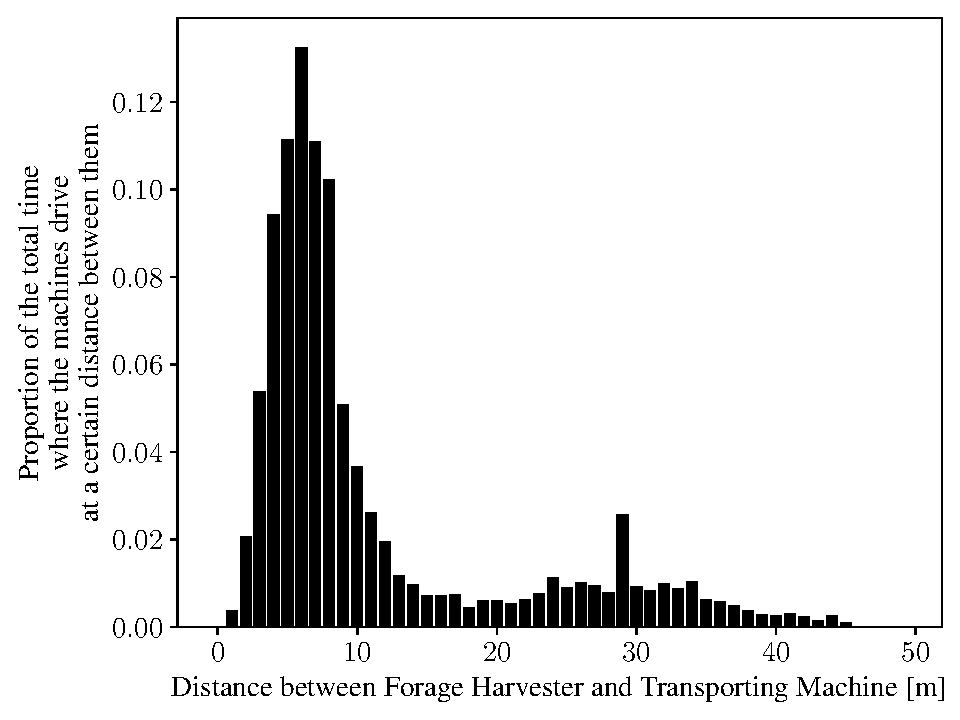
\includegraphics[width=0.85\textwidth]{figures/distanceHarvestSzenario.pdf}
	\caption{Distribution of time proportions where a given distance was between \ac{FH} and \ac{TM} in a harvest platoon scenario.}%
	\label{fig:distance}%
\end{figure}
\begin{figure}%
	\centering
	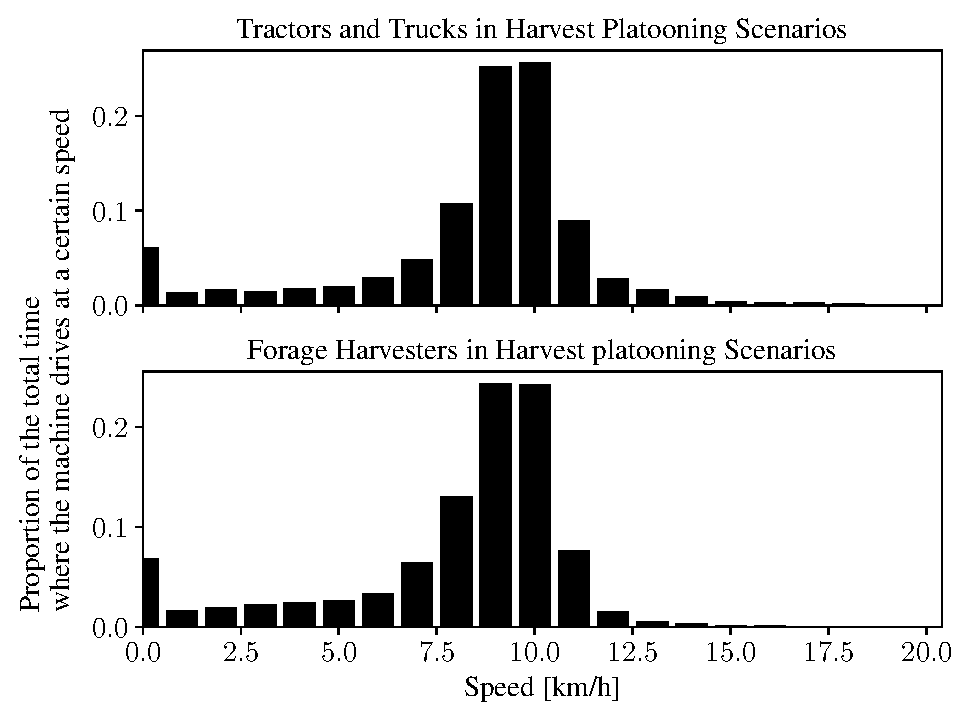
\includegraphics[width=0.85\textwidth]{figures/speedHarvestSzenario.pdf}
	\caption{Distribution of time proportions where \ac{FH} and \ac{TM} drove with a certain speed in a harvest platoon scenario}%
	\label{fig:speed}%
\end{figure}

After the platoons scenarios were correctly detected, I included the data points before each platoons scenario till a maximum distance of \SI{50}{\metre} between \ac{FH} and \ac{TM} was exceeded. These data points are also relevant to the requirements because at the beginning of an agricultural platooning service, the \ac{FH}, as the leader of the system, must be able to guide an empty \ac{TM} to the appropriate position for overloading.

For the detected data points of the platooning services from recorded data of the corn harvest, the proportion where the \ac{FH} and \ac{TM} move in a specific distance is shown in \autoref{fig:distance}. For the same data points, the proportion in which \ac{FH} and \ac{TM} move at a given speed is available in \autoref{fig:speed}.

These analysing results show that the \ac{TM} and the \ac{FH} usually move with a distance of less than \SI{10}{\metre}. In addition, the distance can also be higher, e.g. in turning manoeuvres or before the overloading process.

\textcite{IVAN} gibt in der Zielstellung die für die Entwicklung von Platooning Services im Corn harvest process a distance of less  than \SI{30}{\metre}.


One notable observation in \autoref{fig:speed} is that the \ac{FH} and \ac{TM}s in the corn harvesting platooning scenario often travel at a speed of approximately \SI{10}{\kilo\metre\per\hour}. This speed is significantly higher than the average speed of \SI{5.6}{\kilo\metre\per\hour} of a \ac{FH} in an entire corn harvesting process from \cite{faustzahlen2018}. It is necessary to classify that in the year of the recorded data was little precipitation, so the corn was not dense and high, and the last speed value is an average value of the entire corn harvest process, which can be calculated from the data in \cite{faustzahlen2018}.
Nevertheless, the recorded data shows that a platooning service in agriculture must also be designed for higher speeds. 

\textcite{IVAN} gibt in der Zielstellung die für die Entwicklung von Platooning Services im Corn harvest process einen average speed of \SI{4.5}{\kilo\metre\per\hour}. Je nach \ac{PPD} kann die Geschwindigkeit nach den Autoren von \SIrange{2}{6}{\kilo\metre\per\hour} schwanken. 


\textcite{klingler_agriculture_2018} investigated the suitability of IEEE 802.11p for \ac{WIC}. The authors detected that shadowing effects occur in the harvest scenario. The authors explain the effect because another tractor or the spout of the \ac{FH} was in \ac{LOS}.
\begin{figure}%
	\centering
	\begin{tikzpicture}
		\node[label=below right:FH](a) at (0,0) {\textbullet};
		\node[label=above:North](d) at (0,1) {\textbullet};
		\node[label=above:Heading](c) at (1,1.5) {\textbullet};
		\node[label=below:TM](b) at (2,0) {\textbullet};
		\node[label=below:FHprev](e) at (-1,-1.5) {\textbullet};
		\node[label=above:North](f) at (-1,-0.5) {\textbullet};
		\draw [thick] (a) -- (b);
		\draw [thick] (a) -- (c);
		\draw [thick] (a) -- (d);
		\draw [thick] (a) -- (e);
		\draw [thick] (e) -- (f);
		\draw 
		pic["$\beta$", draw, <-,angle eccentricity=0.8, angle radius=1.0cm]
		{angle=b--a--d}
		pic["$\alpha$", draw, <-,angle eccentricity=1.2, angle radius=1.0cm]
		{angle=a--e--f}
		pic["$Relative Bearing$", draw, <-, angle eccentricity=1.7, angle radius=1.5cm]
		{angle=b--a--c};
	\end{tikzpicture}
	\caption{Relative bearing between \ac{FH} and \ac{TM} which is calculated using the previous location of \ac{FH} by using $\beta$ and $\alpha$ for \autoref{eq:RelativeBearing}}%
	\label{fig:bearing_fh_tm}%
\end{figure}
I reviewed the recorded position data to get an overview of where a \ac{TM} is in the overloading process relative to the \ac{FH}. The relative bearing is the angle between B and the heading of point A. Using the previous position of the \ac{FH}, the relative bearing between \ac{FH} and \ac{TM} can be calculated with the angles $\alpha$ and $\beta$ in \autoref{fig:bearing_fh_tm} as:
\begin{equation}\label{eq:RelativeBearing}
	Relative\_Bearing = \beta - \alpha	,
\end{equation}
Assuming that the \ac{FH} does not move backwards, we can see from the relative bearing in which angle from the \ac{FH} the \ac{TM} is located. The result is displayed in \autoref{fig:bearing}. It can be observed that the \ac{TM} is mainly close to the \ac{FH} at an angle of \SIrange{30}{150}{\degree} at a distance between \SIrange{0}{10}{\metre}. 

In addition, it is noticeable that the machine can also be directly behind the \ac{FH}. This driving behind each other is common when a new part of the field is being cut in harvesting, as can be seen in \autoref{fig:startpart}. When there is a greater distance between \ac{TM} and \ac{FH}, the \ac{TM} is usually behind the FH at a angle of \SIrange{157.5}{187.5}{\degree}. At these moments, the \ac{TM} is empty and closes up to the \ac{FH} to operate in a new platooning Service together. 

\begin{figure}%
	\centering
	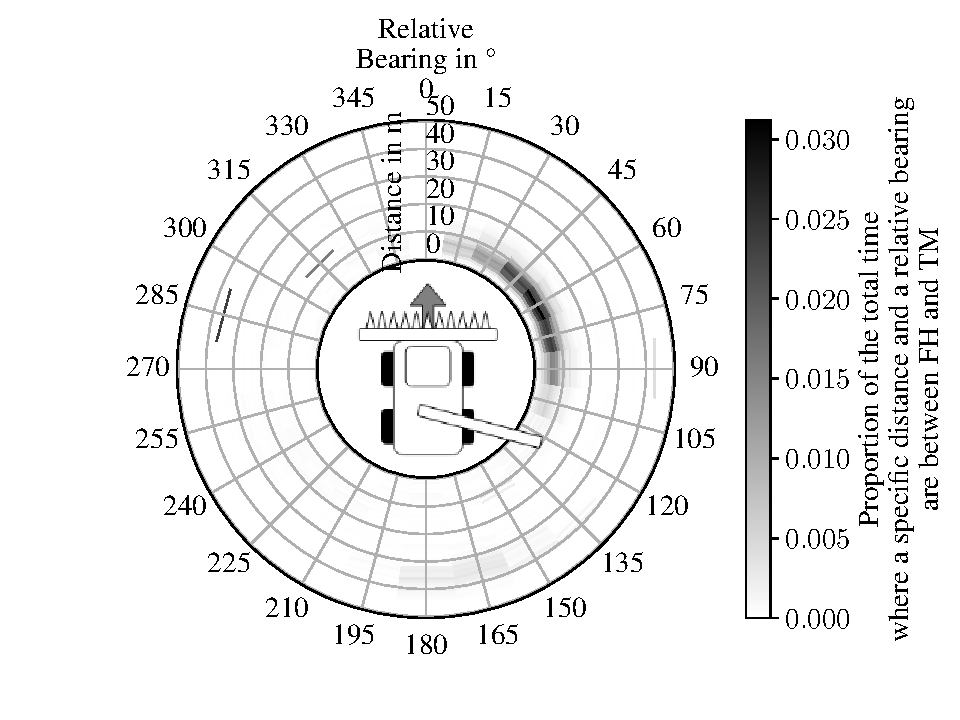
\includegraphics[width=0.99\textwidth]{figures/bearingHarvestScenario50.pdf}
	\caption{Distribution of time proportion at specific distances and relative bearings between \ac{FH} and \ac{TM}}%
	\label{fig:bearing}%
\end{figure}

\begin{figure}%
	\centering
	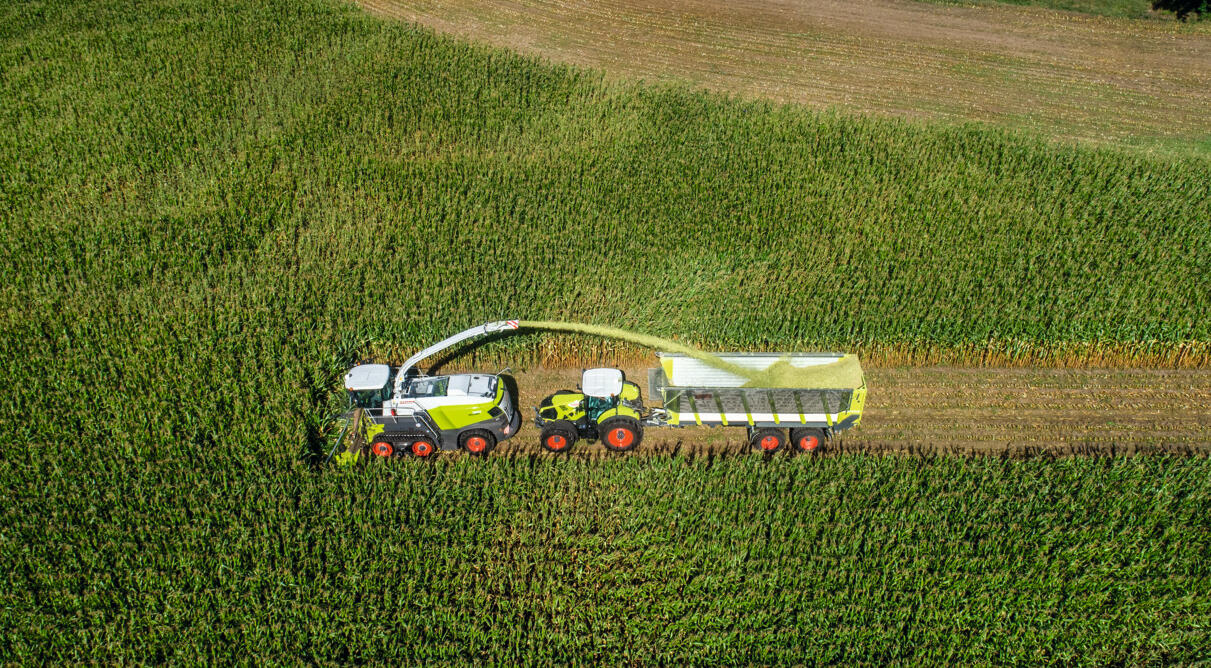
\includegraphics[width=0.8\textwidth]{figures/claas_harvest_behind.png}
	\caption{\ac{FH} and \ac{TM} start cutting a new field section}%
	\label{fig:startpart}%
\end{figure}

Another notable fact is that the \ac{TM} hardly ever stayed to the left of the \ac{FH}. Since the \ac{FH} often made left turns, the crop was usually already harvested to the right of the \ac{FH} so that the \ac{TM} could drive there without running over the crop. On rare occasions, the \ac{TM} was also to the left of the \ac{FH}. Such a platooning scenario can be an exception or a driving manoeuvrer to start cutting a new part of the field.   

The results reveal only a first impression of the requirements of a harvest and loading process. More data from around the world needs to be analyzed to make a general statement. The low rainfall this year has already set a low plant population. This field condition made a higher process speed possible. To make a general statement, I should use data from different years because they can reveal different initial field conditions.



\TODO{
	Heading Annahme Vorwärts Fahrt. Ansonsten Überprüfen und nochmal Einzelfahrt plotten und anschauen. 
	Wie oft dreht sich das Heading ?
	Möglicherweise Rückwärtsfahrt erkennen? Oder WIC Requirements erwähnen? }
